%%=============================================================================
%% Conclusie
%%=============================================================================

\chapter{Conclusie}%
\label{ch:conclusie}

\section{Resultaten}
De ontwikkeling en evaluatie van het LSTM-model voor het voorspellen van energieverbruik en het detecteren van anomalieën bij de ovens van ArcelorMittal hebben cruciale inzichten opgeleverd. Het model, bestaande uit drie lagen met respectievelijk 256, 128, en 64 units gevolgd door een Dense output laag, is uitvoerig getest en geëvalueerd. Uit deze evaluatie bleek dat een sequence length van 64 optimaal was, wat resulteerde in een validation loss van 0.023. Dit toont aan dat het model effectief is in het identificeren van patronen in tijdreeksdata en het voorspellen van energieverbruik met hoge nauwkeurigheid.

\section{Modelprestaties}
De prestaties van het LSTM-model overtreffen die van traditionele machine learning-modellen zoals lineaire regressie, beslisbomen, en random forests die ook getest werden. Deze resultaten onderstrepen het vermogen van geavanceerde deep learning technieken om complexe, dynamische systemen zoals industriële ovens te modelleren, wat een significante verbetering is ten opzichte van meer traditionele methoden.

\section{Vergelijking met andere modellen}
Hoewel alternatieve machine learning-algoritmen bepaalde niveaus van voorspellingsnauwkeurigheid boden, bevestigde de experimentatie dat de LSTM-structuur aanzienlijk betere resultaten leverde, vooral in de context van sequentiële en tijd-afhankelijke data zoals die van ArcelorMittal's productieprocessen.

\section{Implicaties en toepassingen}
De bevindingen van dit onderzoek hebben directe implicaties voor het energiemanagement binnen ArcelorMittal. Door nauwkeurige voorspellingen en tijdige detectie van anomalieën kan het bedrijf aanzienlijke energiebesparingen realiseren, wat leidt tot kostenreductie en een vermindering van de ecologische voetafdruk. Deze modellen bieden ook een waardevolle tool voor andere industriële toepassingen waar energiemanagement een prioriteit is.

\section{Aanbevelingen voor toekomstig onderzoek}
Het is aan te bevelen dat toekomstig onderzoek zich richt op de integratie van real-time data feeds om het model in staat te stellen dynamische aanpassingen te maken in respons op onmiddellijke operationele veranderingen. Verder zou de exploratie van hybride modellen die LSTM combineren met andere voorspellende technieken, zoals convolutionele neurale netwerken (CNNs), kunnen leiden tot nog accuratere en robuustere voorspellingssystemen.

\section{Conclusie}
Samenvattend heeft deze studie aangetoond dat geavanceerde machine learning-modellen zoals LSTM's effectief kunnen worden ingezet om het energieverbruik in complexe industriële omgevingen te voorspellen en te optimaliseren. De resultaten van deze bachelorproef bieden niet alleen een basis voor operationele verbeteringen bij ArcelorMittal maar dragen ook bij aan de bredere kennisbasis over energie-efficiëntie en duurzaamheidsinitiatieven binnen de industrie.

\subsection{Visualisaties}
\begin{figure}[h!]
    \centering
    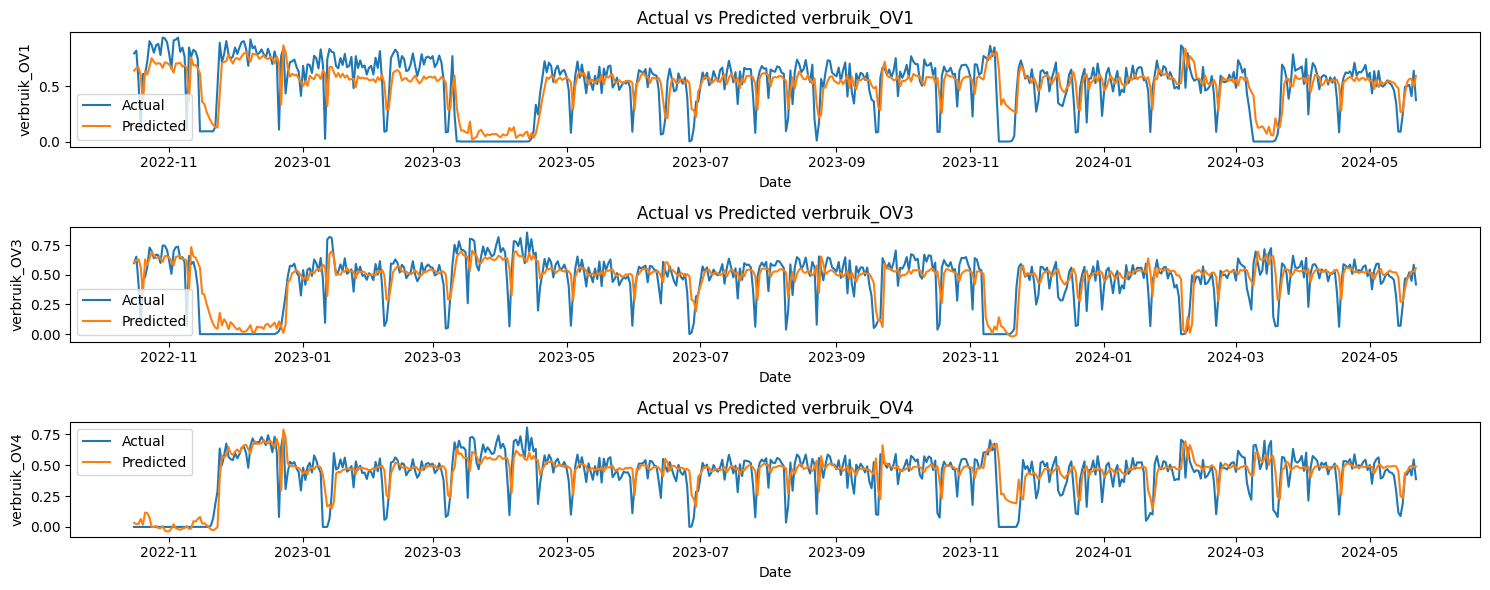
\includegraphics[width=\textwidth]{graphics/ActualVSPredicted.png}
    \caption{Effectief verbruik versus voorspeld verbruik van het model voor alle drie de ovens.}
    \label{fig:ActualVSPredicted}
\end{figure}
